\documentclass[10pt]{article}
\usepackage[a4paper,margin=0.85in]{geometry}
\usepackage[T1]{fontenc}
\usepackage{amsmath,amssymb,graphicx,booktabs}
\usepackage[hidelinks]{hyperref}
\usepackage{microtype}
\usepackage{xcolor}
\setlength{\parindent}{0pt}
\setlength{\parskip}{0.65em}
\title{Supplemental Material for ``Self-similar Worthington jets''}
\author{Jos\'e M. Gordillo, Javier Rodr\'iguez--Rodr\'iguez, and Vatsal Sanjay}
\date{}
\renewcommand{\thefigure}{S\arabic{figure}}
\begin{document}
\maketitle

\section*{Cone-angle extraction and sensitivity}

At the snapshot nearest to jet inception, we fit the cavity flank to $r_p=mz'+c$ by unweighted least squares on the interface-facet endpoints within $-1.30\le z'\le-0.25$ and $0.20\le r_p\le1.10$ (Fig.~\ref{fig:cone-sensitivity}(a)). The fitted line gives the semiangle from the axis, $\beta=\arctan m$, and the apparent apex, $\ell_0=-c/m$. This full-window fit gives $\beta=38.356^\circ$. Solving $P_\nu(-\cos\beta)=0$ then determines $\alpha=1/(2-\nu)$ independently of the jet-flux fit.

\begin{figure}[!ht]
\centering
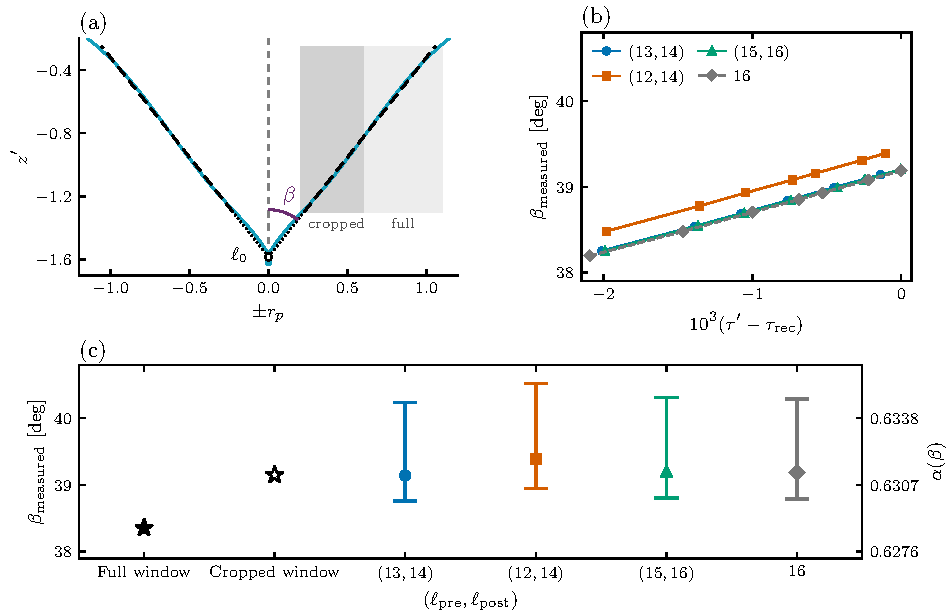
\includegraphics[width=\textwidth]{supplemental-figures/cone-fit-sensitivity-v4.pdf}
\caption{Cone-angle extraction and sensitivity. (a) Cavity interface at $Oh=0.03$, with the full fitting window in light grey and its cropped part in darker grey. The full-window fit (dashed line) gives $\beta=38.4^\circ$; dotted extensions reach the apparent apex $\ell_0$, and the arc measures $\beta$ from the axis. (b) Evolution of $\beta$ before reconnection, using the cropped window at the available snapshot times. (c) Angles at the last pre-reconnection snapshot of each simulation, labelled by pre/post refinement levels, with ranges from nine fitting windows. The right axis gives the corresponding $\alpha(\beta)$. Filled and open stars mark the full and cropped fits to the same interface in (a).}
\label{fig:cone-sensitivity}
\end{figure}

To compare with the other interface sequences, which extend only to $r_p<0.6$, we crop the radial fitting window to $0.20\le r_p\le0.60$ and retain the same axial limits. For the same interface in Fig.~\ref{fig:cone-sensitivity}(a), cropping alone increases $\beta$ to $39.151^\circ$, a shift of $0.795^\circ$. Within the cropped window, $\beta$ rises by $0.89$--$0.99^\circ$ during the last $\tau \approx 2\times10^{-3}$ before reconnection (Fig.~\ref{fig:cone-sensitivity}(b)). Across the nine windows defined by $r_{p,\min}\in\{0.15,0.20,0.25\}$ and $r_{p,\max}\in\{0.50,0.55,0.60\}$, the fitted angle varies by $1.48$--$1.57^\circ$ at the last pre-reconnection snapshot of each simulation (panel c).

The solver, cone-fitting routine and paper-processing scripts are available in the \href{https://github.com/comphy-lab/Bursting-Bubble}{public CoMPhy Lab repository}.

\section*{Flux exponents and refinement}

At $Oh=0.03$, the jet has $We_j\simeq80$--$142$ and $Re_j\simeq23$--$51$ over the reference interval $0.005\le r_j\le0.023952$. The Weber number is large and increases as $r_j$ decreases; together with $Re_j>20$, this supports the inertial balance within this window. We take the theoretical exponent $0.629$ from the cone geometry and compare it with the numerical flux slopes measured independently over finite radius intervals.

For a flux law $Q_j\propto r_j^s$, the corresponding Weber-number law is $We_j\propto r_j^{2s-3}$ and the effective exponent is $\alpha_{\rm eff}=1/(3-s)$. The two slopes are therefore algebraically equivalent diagnostics. We fit the plotted jet-base flux $Q_j$ separately for each refinement history $(\ell_{\rm pre},\ell_{\rm post})$, keeping histories with the same final level distinct. For each trajectory, the fit uses geometric means from 24 equal logarithmic radius bins, with equal weight assigned to every occupied bin.

We compare fixed exponents by refitting their amplitudes on the same observations, with equal total weight per occupied radius bin. The smaller residuals for $0.629$ than for $2/3$ in all nine tested windows for each of the nine available histories favour $0.629$ over these intervals.

\begin{table}[ht]
\centering
\begin{tabular}{ccccc}
\toprule
$(\ell_{\rm pre},\ell_{\rm post})$ & $s$ & $\alpha_{\rm eff}$ & RMS ($0.629$) & RMS ($2/3$)\\
\midrule
(12,13) & $1.4472\pm0.0026$ & $0.6440\pm0.0011$ & 0.01772 & 0.02501\\
(12,14) & $1.4254\pm0.0038$ & $0.6351\pm0.0015$ & 0.00852 & 0.03381\\
(13,14) & $1.4320\pm0.0025$ & $0.6378\pm0.0010$ & 0.01083 & 0.03205\\
(13,15) & $1.4231\pm0.0021$ & $0.6342\pm0.0009$ & 0.00675 & 0.03615\\
(14,15) & $1.4063\pm0.0039$ & $0.6275\pm0.0015$ & 0.00749 & 0.04240\\
(14,16) & $1.4102\pm0.0036$ & $0.6290\pm0.0014$ & 0.00485 & 0.04049\\
(15,15) & $1.4031\pm0.0036$ & $0.6262\pm0.0014$ & 0.00835 & 0.04454\\
(15,16) & $1.4025\pm0.0052$ & $0.6260\pm0.0021$ & 0.00914 & 0.04957\\
(16,16) & $1.3998\pm0.0039$ & $0.6249\pm0.0015$ & 0.00897 & 0.04544\\
\bottomrule
\end{tabular}
\caption{Finite-window flux fits at $Oh=0.03$, reconstructed from the plotted observations. The reference window contains 11--25 observations and 11--24 occupied bins per trajectory. The quoted uncertainties are formal least-squares residual standard errors, calculated with $m-2$ degrees of freedom for $m$ occupied bins. The last two columns give the RMS residual in $\ln Q_j$ for the fixed exponents $\alpha=0.629$ and $\alpha=2/3$. For each fixed exponent, the amplitude is refitted to the same extracted observations, with equal total weight assigned to each occupied radius bin.}
\label{tab:flux}
\end{table}

Leaving the slope free gives $0.6249\le\alpha_{\rm eff}\le0.6290$ for the five histories with $\ell_{\rm pre}\ge14$ in the reference window, close to the value selected by the cone geometry. For $(\ell_{\rm pre},\ell_{\rm post})=(16,16)$, however, varying the fitting window gives $0.6118\le\alpha_{\rm eff}\le0.6304$ (Table~\ref{tab:windows}). The small formal errors are derived from residual scatter within individual fits and account for neither window dependence nor correlations along a trajectory.

\begin{table}[ht]
\centering
\small
\begin{tabular}{cccccc}
\toprule
$r_{j,\min}$ & $r_{j,\max}$ & $(12,13)$ & $(12,14)$ & $(13,14)$ & $(13,15)$\\
\midrule
0.0050 & 0.018000 & 0.6465 & 0.6389 & 0.6403 & 0.6362\\
0.0050 & 0.023952 & 0.6440 & 0.6351 & 0.6378 & 0.6342\\
0.0050 & 0.030000 & 0.6401 & 0.6298 & 0.6333 & 0.6301\\
0.0065 & 0.018000 & 0.6458 & 0.6356 & 0.6399 & 0.6365\\
0.0065 & 0.023952 & 0.6424 & 0.6306 & 0.6364 & 0.6333\\
0.0065 & 0.030000 & 0.6376 & 0.6241 & 0.6308 & 0.6280\\
0.0080 & 0.018000 & 0.6436 & 0.6336 & 0.6380 & 0.6356\\
0.0080 & 0.023952 & 0.6396 & 0.6285 & 0.6336 & 0.6312\\
0.0080 & 0.030000 & 0.6340 & 0.6217 & 0.6269 & 0.6246\\
\bottomrule
\end{tabular}
\par
\medskip
\begin{tabular}{ccccccc}
\toprule
$r_{j,\min}$ & $r_{j,\max}$ & $(14,15)$ & $(14,16)$ & $(15,15)$ & $(15,16)$ & $(16,16)$\\
\midrule
0.0050 & 0.018000 & 0.6319 & 0.6327 & 0.6313 & 0.6310 & 0.6304\\
0.0050 & 0.023952 & 0.6275 & 0.6290 & 0.6262 & 0.6260 & 0.6249\\
0.0050 & 0.030000 & 0.6229 & 0.6235 & 0.6217 & 0.6218 & 0.6197\\
0.0065 & 0.018000 & 0.6287 & 0.6305 & 0.6277 & 0.6277 & 0.6275\\
0.0065 & 0.023952 & 0.6241 & 0.6252 & 0.6215 & 0.6211 & 0.6209\\
0.0065 & 0.030000 & 0.6191 & 0.6180 & 0.6177 & 0.6173 & 0.6148\\
0.0080 & 0.018000 & 0.6250 & 0.6290 & 0.6248 & 0.6256 & 0.6254\\
0.0080 & 0.023952 & 0.6200 & 0.6232 & 0.6191 & 0.6185 & 0.6183\\
0.0080 & 0.030000 & 0.6148 & 0.6155 & 0.6140 & 0.6144 & 0.6118\\
\bottomrule
\end{tabular}
\caption{Effective exponents $\alpha_{\rm eff}$ obtained by varying the radius window, using the same 24-bin fitting procedure for each refinement history. Column headings give $(\ell_{\rm pre},\ell_{\rm post})$. Together, the two blocks contain the nine histories for which flux observations at $Oh=0.03$ are available in the figure.}
\label{tab:windows}
\end{table}

\section*{Radius at a fixed Reynolds number}

For the singular Worthington jet, a natural continuum cutoff may come from viscous stresses. However, the simulations do not resolve that cutoff length scale $r_j = r_m$, such that $Re_j \equiv v_jr_j/Oh \sim 1$. We compare the resolved jet across $Oh$ using its radius $r_j(Re_*)$ when the jet-base Reynolds number $Re_j$ reaches $Re_*=20$, 25 or 30. For a fixed cone angle, $v_jr_j\propto r_j^{(2\alpha-1)/\alpha}$ gives $r_j(Re_*)\propto(Re_*Oh)^{\alpha/(2\alpha-1)}$, so these choices alter the prefactor without changing the predicted power of $Oh$.

We first take the median $Re_j$ within logarithmically spaced radius bins to suppress isolated transient spikes. We then interpolate in logarithmic coordinates between the two bin medians bracketing $Re_*$ to obtain $r_j(Re_*)$, using the same procedure for every $Oh$ and refinement history. For $Re_*=20$, the $(15,15)$ and $(16,16)$ histories give almost identical radii at $Oh=0.03$ and differ by about six percent at $Oh=0.04$ (Fig.~\ref{fig:threshold}). The corresponding radii at $Re_*=25$ and 30 also increase with $Oh$, while the differences between these two histories remain small. Neither the increase above the low-$Oh$ plateau nor the agreement between these histories therefore depends on choosing $Re_*=20$.

\begin{figure}[ht]
\centering
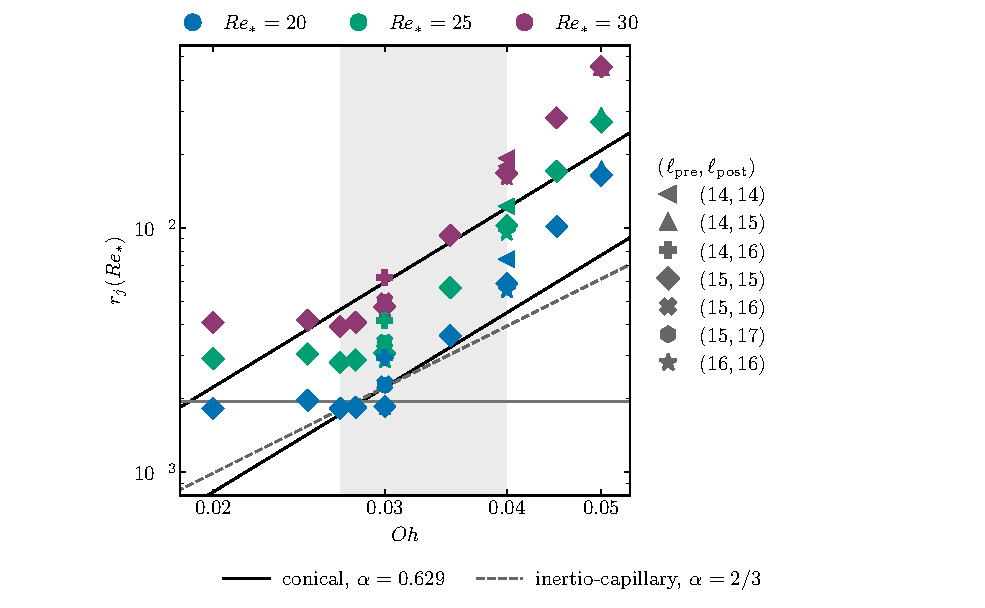
\includegraphics[width=\textwidth]{supplemental-figures/reynolds-threshold-sensitivity-v7.pdf}
\caption{Jet radius $r_j(Re_*)$ versus $Oh$ at $Re_*=20$ (blue), 25 (green) and 30 (purple), with symbols identifying the refinement pairs $(\ell_{\mathrm{pre}},\ell_{\mathrm{post}})$. Solid black lines show the conical scaling at $Re_*=20$ (lower) and 30 (upper), and the grey dashed line shows the inertio-capillary scaling. The horizontal grey line indicates the low-$Oh$ plateau, and the shaded band covers the conical regime $0.027<Oh<0.04$. The $Re_*=20$ points and guides are the same as in the inset of Fig.~2(b) and Fig.~5(c) of the Letter.}
\label{fig:threshold}
\end{figure}

\section*{Interface collapse}

Figure~\ref{fig:collapse-comparison} compares the profiles shown in Fig.~3 of the Letter after rescaling with $\alpha=2/3$ and $\alpha=0.629$. Both exponents collapse the interfaces over the displayed pre- and post-inception windows, so the collapse of the shapes alone does not distinguish the underlying force balance.

\begin{figure}[ht]
\centering
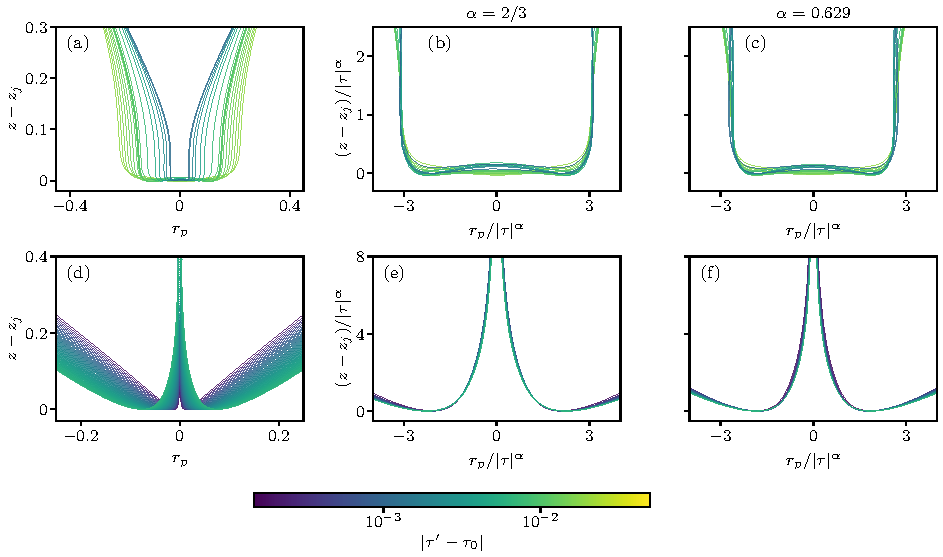
\includegraphics[width=\textwidth]{supplemental-figures/interface-collapse-comparison-v1.pdf}
\caption{Comparison of the two similarity exponents on the same interfaces. The upper row shows pre-inception cavity collapse; the lower row shows the post-inception jet. Columns show unscaled profiles, $\alpha=2/3$, and $\alpha=0.629$. In each rescaled panel, $\tau=\tau'-\tau_0$, with $\tau_0=0.494430$. Supplementary Videos~1 and~2 show the pre- and post-inception sequences.}
\label{fig:collapse-comparison}
\end{figure}

\section*{Supplementary videos}
Video~1 shows the pre-inception cavity.\\
Video~2 shows the post-inception jet.\\
Video~3 provides a visual summary of the work.\\
Files: \texttt{SM1-pre-collapse.mp4}, \texttt{SM2-post-collapse.mp4}, and \texttt{SM3-summary.mp4}.

\end{document}
